% -*- mode: latex; -*- mustache tags:  
\documentclass[10pt,twoside,english]{_support/latex/sbabook/sbabook}
\let\wholebook=\relax

\usepackage{amsmath}

\usepackage{import}
\subimport{_support/latex/}{common.tex}

%=================================================================
% Debug packages for page layout and overfull lines
% Remove the showtrims document option before printing
\ifshowtrims
  \usepackage{showframe}
  \usepackage[color=magenta,width=5mm]{_support/latex/overcolored}
\fi


% =================================================================
\title{The Pillar Super BOD Book Archetype Using Microdown}
\author{The Pillar team}
\series{Square Bracket tutorials}

\hypersetup{
  pdftitle = {The Pillar Super BOD Book Archetype Using Microdown},
  pdfauthor = {The Pillar team},
  pdfkeywords = {project template, Pillar, Pharo, Smalltalk}
}


% =================================================================
\begin{document}

\newpage
\thispagestyle{empty}
\mbox{}
\newpage
\thispagestyle{empty}
\mbox{}

% Title page and colophon on verso
\maketitle
\pagestyle{titlingpage}
\thispagestyle{titlingpage} % \pagestyle does not work on the first one…

\cleartoverso
{\small

  Copyright 2023 by The Pillar team.

  The contents of this book are protected under the Creative Commons
  Attribution-NonCommercial-NoDerivs 
  CC BY-NC-ND\\
You are free to:
\begin{description}
\item Share --- copy and redistribute the material in any medium or format
\end{description}

The licensor cannot revoke these freedoms as long as you follow the license terms.
  Under the following conditions:
  \begin{description}
  \item[Attribution.] ---  You must give appropriate credit, provide a link to the license, and indicate if changes were made. You may do so in any reasonable manner, but not in any way that suggests the licensor endorses you or your use.
\item[NonCommercial.] ---  You may not use the material for commercial purposes.
\item [NoDerivatives.] ---  If you remix, transform, or build upon the material, you may not distribute the modified material.
\item [No additional restrictions.] ---  You may not apply legal terms or technological measures that legally restrict others from doing anything the license permits.
  \end{description}

\url{https://creativecommons.org/licenses/by-nc-nd/4.0/legalcode}

Any of the above conditions can be waived if you get permission from
the copyright holder. Nothing in this license impairs or restricts the
author's moral rights.

\begin{center}
    
\includegraphics[width=0.2\textwidth]{_support/latex/CreativeCommons-BYNOCND.pdf}
\end{center}

  \vfill
Keepers of the lighthouse\\
Édition : BoD - Books on Demand,\\
12/14 rond-point des Champs-Élysées,75008 Paris\\
Impression : Books on Demand GmbH, Norderstedt, Allemagne\\
ISBN: XXXXXXXXXXXXXXX\\
Dépôt légal : Month/YEAR\\
Layout and typography based on the \textcode{sbabook} \LaTeX{} class by Damien Pollet.
}


\frontmatter
\pagestyle{plain}

\tableofcontents*
%\clearpage\listoffigures

\mainmatter


\part{My First book using Microdown}
\chapter{Compilation}
\begin{figure}[htpb]
\begin{center}

\includegraphics[width=0.3\textwidth]{/Users/ducasse/Workspace/FirstCircle/MyBooks/Bk-Writing/PharoBooks2/booklet-template/Chapters/Chapter1/figures/pillar.png}
\caption{Pillar logo}\label{fig}
\end{center}
\end{figure}


\section{Welcome to Pillar's little user-guide !!}
To write a book, you can create chapters and include them into \textcode{book.pillar}
or directly edit the file.
If you don't know ''Pillar'', check its documentation at \href{}{\href{http://github.com/pillar-markup/pillar}{http://github.com/pillar-markup/pillar}}

\chapter{Edition and Templates}
There is also a template system, you can find template in the folder \textcode{\_support/template}.
Some template are already written, but if you want to have your own, you had two solutions:

\begin{itemize}
    \item edit the existing template related to the format you want to change (recommanded)
    \item create your own template with its own name
\end{itemize}

You will found some template examples in \textcode{\_support/template} folder to see how it works.
The default template system is Mustache.

Output directory's default name is ''book-result'' but you can change it in the pillar.conf file by editing the\textcode{OUTPUTDIRECTORY} variable

\begin{figure}[htpb]
\begin{center}

\includegraphics[width=0.3\textwidth]{/Users/ducasse/Workspace/FirstCircle/MyBooks/Bk-Writing/PharoBooks2/booklet-template/Chapters/Chapter2/figures/pharo.png}
\caption{blue}
\end{center}
\end{figure}
\begin{figure}[htpb]
\begin{center}
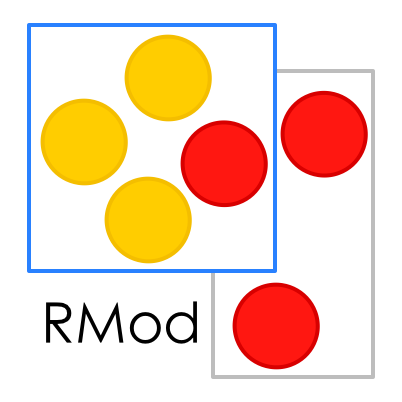
\includegraphics[width=0.3\textwidth]{/Users/ducasse/Workspace/FirstCircle/MyBooks/Bk-Writing/PharoBooks2/booklet-template/Chapters/Chapter2/figures/rmod.png}
\caption{jlklkjlk}
\end{center}
\end{figure}



% lulu requires an empty page at the end. That's why I'm using
% \backmatter here.
\backmatter

% Index would go here

\end{document}
